%%%%%%%%%%%%%%%%%%%%%%%%%%%%%%%%%%%%%%%%%
% Masters/Doctoral Thesis 
% LaTeX Template
% Version 2.5 (27/8/17)
%
% This template was downloaded from:
% http://www.LaTeXTemplates.com
%
% Version 2.x major modifications by:
% Vel (vel@latextemplates.com)
%
% This template is based on a template by:
% Steve Gunn (http://users.ecs.soton.ac.uk/srg/softwaretools/document/templates/)
% Sunil Patel (http://www.sunilpatel.co.uk/thesis-template/)
%
% Template license:
% CC BY-NC-SA 3.0 (http://creativecommons.org/licenses/by-nc-sa/3.0/)
%
%%%%%%%%%%%%%%%%%%%%%%%%%%%%%%%%%%%%%%%%%

%----------------------------------------------------------------------------------------
%	PACKAGES AND OTHER DOCUMENT CONFIGURATIONS
%----------------------------------------------------------------------------------------

\documentclass[
11pt, % The default document font size, options: 10pt, 11pt, 12pt
%oneside, % Two side (alternating margins) for binding by default, uncomment to switch to one side
english, % ngerman for German
singlespacing, % Single line spacing, alternatives: onehalfspacing or doublespacing
%draft, % Uncomment to enable draft mode (no pictures, no links, overfull hboxes indicated)
%nolistspacing, % If the document is onehalfspacing or doublespacing, uncomment this to set spacing in lists to single
%liststotoc, % Uncomment to add the list of figures/tables/etc to the table of contents
%toctotoc, % Uncomment to add the main table of contents to the table of contents
%parskip, % Uncomment to add space between paragraphs
%nohyperref, % Uncomment to not load the hyperref package
headsepline, % Uncomment to get a line under the header
%chapterinoneline, % Uncomment to place the chapter title next to the number on one line
%consistentlayout, % Uncomment to change the layout of the declaration, abstract and acknowledgements pages to match the default layout
]{MastersDoctoralThesis} % The class file specifying the document structure

\usepackage[utf8]{inputenc} % Required for inputting international characters
\usepackage[T1]{fontenc} % Output font encoding for international characters

\usepackage{mathpazo} % Use the Palatino font by default

\usepackage[backend=bibtex,style=authoryear,natbib=true]{biblatex} % Use the bibtex backend with the authoryear citation style (which resembles APA)

\addbibresource{example.bib} % The filename of the bibliography

\usepackage[autostyle=true]{csquotes} % Required to generate language-dependent quotes in the bibliography

\usepackage{color}
\usepackage[normalem]{ulem}
\usepackage{soul} % use this for strikethrough
\newcommand{\mpcomment}[1]{\textcolor{blue}{#1}}
\newcommand{\mpswap}[2]{\st{#1}\textcolor{magenta}{#2}}
%%%%
\usepackage{amsfonts}
\usepackage{amssymb}
\usepackage{amsmath}
\usepackage{mathtools}
\usepackage{upgreek}
\usepackage{color}
\usepackage{changepage}
\usepackage{graphicx}
\usepackage{listings}
\usepackage{multirow}% http://ctan.org/pkg/multirow
\usepackage{hhline}% http://ctan.org/pkg/hhline
\usepackage{mleftright}
\usepackage{float}
\usepackage{mathrsfs}
\usepackage{csquotes}
 
 
\definecolor{mygreen}{RGB}{28,172,0} % color values Red, Green, Blue
\definecolor{mylilas}{RGB}{170,55,241}

\newcommand{\Tau}{\mathrm{T}}
\newcommand{\Lc}{\mathcal{L}}

\def\|{\,|\,}
\def\Z{{\mathbb Z}}
\def\Q{{\mathbb Q}}
\def\C{{\mathbb C}}
\def\grad{{\nabla}}
\def\R{{\mathbb R}}
\def\H{{\mathbb H}}
\def\N{{\mathbb N}}
\def\lams{{\lambda ^*}}
\def\M{{\mathcal M}}
\def\dlam{{d \lambda}}
\def\mubar{{\overline{\mu}}}
\def\Mbar{{\overline{\mathcal{M}}}}
\def\sigmaalgebra{{\sigma\text{-algebra}}}
\def\changemargin#1#2{\list{}{\rightmargin#2\leftmargin#1}\item[]}
\def\mytau{{\uptau}}

\newcommand{\cupti}[1]{\bigcup_{#1=1}^{\infty}}
\newcommand{\capti}[1]{\bigcap_{#1=1}^{\infty}}
\newcommand{\lti}[1]{\lim\limits_{#1\to\infty}}
\newcommand{\sumi}[1]{\sum_{#1}^{\infty}}
\newcommand{\inthigh}[2]{\int\limits_{#1}^{#2}}
\newcommand{\pd}[3]{\frac{\partial^{#1} #2}{\partial {#3}^{#1}}}
\newcommand\tab[1][1cm]{\hspace*{#1}}

%----------------------------------------------------------------------------------------
%	MARGIN SETTINGS
%----------------------------------------------------------------------------------------

\geometry{
	paper=letterpaper, % Change to letterpaper for US letter
	inner=2.5cm, % Inner margin
	outer=3.8cm, % Outer margin
	bindingoffset=.5cm, % Binding offset
	top=1.5cm, % Top margin
	bottom=1.5cm, % Bottom margin
	%showframe, % Uncomment to show how the type block is set on the page
}

%----------------------------------------------------------------------------------------
%	THESIS INFORMATION
%----------------------------------------------------------------------------------------

\thesistitle{Something} % Your thesis title, this is used in the title and abstract, print it elsewhere with \ttitle
\supervisor{Dr. Malgorzata Peszynska } % Your supervisor's name, this is used in the title page, print it elsewhere with \supname
\examiner{} % Your examiner's name, this is not currently used anywhere in the template, print it elsewhere with \examname
\degree{Master's of Science in Mathematics} % Your degree name, this is used in the title page and abstract, print it elsewhere with \degreename
\author{John \textsc{Smith}} % Your name, this is used in the title page and abstract, print it elsewhere with \authorname
\addresses{} % Your address, this is not currently used anywhere in the template, print it elsewhere with \addressname

\subject{Mathematics} % Your subject area, this is not currently used anywhere in the template, print it elsewhere with \subjectname
\keywords{} % Keywords for your thesis, this is not currently used anywhere in the template, print it elsewhere with \keywordnames
\university{\href{http://www.oregonstate.edu}{Oregon State University}} % Your university's name and URL, this is used in the title page and abstract, print it elsewhere with \univname
\department{\href{http://math.oregonstate.edud}{Department of Mathematics}} % Your department's name and URL, this is used in the title page and abstract, print it elsewhere with \deptname
\group{\href{http://researchgroup.university.com}{Department of Mathematics}} % Your research group's name and URL, this is used in the title page, print it elsewhere with \groupname
\faculty{\href{http://faculty.university.com}{Faculty Name}} % Your faculty's name and URL, this is used in the title page and abstract, print it elsewhere with \facname

\AtBeginDocument{
\hypersetup{pdftitle=\ttitle} % Set the PDF's title to your title
\hypersetup{pdfauthor=\authorname} % Set the PDF's author to your name
\hypersetup{pdfkeywords=\keywordnames} % Set the PDF's keywords to your keywords
}

\begin{document}

\frontmatter % Use roman page numbering style (i, ii, iii, iv...) for the pre-content pages

\pagestyle{plain} % Default to the plain heading style until the thesis style is called for the body content

%----------------------------------------------------------------------------------------
%	TITLE PAGE
%----------------------------------------------------------------------------------------

\begin{titlepage}
\begin{center}

\vspace*{.06\textheight}
{\scshape\LARGE \univname\par}\vspace{1.5cm} % University name
\textsc{\Large Master's Thesis}\\[0.5cm] % Thesis type

\HRule \\[0.4cm] % Horizontal line
{\huge \bfseries \ttitle\par}\vspace{0.4cm} % Thesis title
\HRule \\[1.5cm] % Horizontal line
 
\begin{minipage}[t]{0.4\textwidth}
\begin{flushleft} \large
\emph{Author:}\\
\href{http://www.johnsmith.com}{\authorname} % Author name - remove the \href bracket to remove the link
\end{flushleft}
\end{minipage}
\begin{minipage}[t]{0.4\textwidth}
\begin{flushright} \large
\emph{Advisor:} \\
\href{http://www.jamessmith.com}{\supname} % Supervisor name - remove the \href bracket to remove the link  
\end{flushright}
\end{minipage}\\[3cm]
 
\vfill

\large \textit{A thesis submitted in fulfillment of the requirements\\ for the degree of \degreename}\\[0.3cm] % University requirement text
\textit{in the}\\[0.4cm]
\deptname\\[2cm] % Research group name and department name
 
\vfill

{\large \today}\\[4cm] % Date
%\includegraphics{Logo} % University/department logo - uncomment to place it
 
\vfill
\end{center}
\end{titlepage}

%----------------------------------------------------------------------------------------
%	DECLARATION PAGE
%----------------------------------------------------------------------------------------

\begin{declaration}
\addchaptertocentry{\authorshipname} % Add the declaration to the table of contents
\noindent I, \authorname, declare that this thesis titled, \enquote{\ttitle} and the work presented in it are my own. I confirm that:

\begin{itemize} 
\item This work was done wholly or mainly while in candidature for a research degree at this University.
\item Where any part of this thesis has previously been submitted for a degree or any other qualification at this University or any other institution, this has been clearly stated.
\item Where I have consulted the published work of others, this is always clearly attributed.
\item Where I have quoted from the work of others, the source is always given. With the exception of such quotations, this thesis is entirely my own work.
\item I have acknowledged all main sources of help.
\item Where the thesis is based on work done by myself jointly with others, I have made clear exactly what was done by others and what I have contributed myself.\\
\end{itemize}
 
\noindent Signed:\\
\rule[0.5em]{25em}{0.5pt} % This prints a line for the signature
 
\noindent Date:\\
\rule[0.5em]{25em}{0.5pt} % This prints a line to write the date
\end{declaration}

\cleardoublepage

% %----------------------------------------------------------------------------------------
% %	QUOTATION PAGE
% %----------------------------------------------------------------------------------------

% \vspace*{0.2\textheight}

% \noindent\enquote{\itshape Thanks to my solid academic training, today I can write hundreds of words on virtually any topic without possessing a shred of information, which is how I got a good job in journalism.}\bigbreak

% \hfill Dave Barry

%----------------------------------------------------------------------------------------
%	ABSTRACT PAGE
%----------------------------------------------------------------------------------------

\begin{abstract}
\addchaptertocentry{\abstractname} % Add the abstract to the table of contents
The Thesis Abstract is written here (and usually kept to just this page). The page is kept centered vertically so can expand into the blank space above the title too\ldots
\end{abstract}

%----------------------------------------------------------------------------------------
%	ACKNOWLEDGEMENTS
%----------------------------------------------------------------------------------------

\begin{acknowledgements}
\addchaptertocentry{\acknowledgementname} % Add the acknowledgements to the table of contents
The acknowledgments and the people to thank go here, don't forget to include your project advisor\ldots
\end{acknowledgements}

%----------------------------------------------------------------------------------------
%	LIST OF CONTENTS/FIGURES/TABLES PAGES
%----------------------------------------------------------------------------------------

\tableofcontents % Prints the main table of contents

\listoffigures % Prints the list of figures

\listoftables % Prints the list of tables

%----------------------------------------------------------------------------------------
%	ABBREVIATIONS
%----------------------------------------------------------------------------------------

\begin{abbreviations}{ll} % Include a list of abbreviations (a table of two columns)

\textbf{LAH} & \textbf{L}ist \textbf{A}bbreviations \textbf{H}ere\\
\textbf{WSF} & \textbf{W}hat (it) \textbf{S}tands \textbf{F}or\\

\end{abbreviations}

%----------------------------------------------------------------------------------------
%	PHYSICAL CONSTANTS/OTHER DEFINITIONS
%----------------------------------------------------------------------------------------

\begin{constants}{lr@{${}={}$}l} % The list of physical constants is a three column table

% The \SI{}{} command is provided by the siunitx package, see its documentation for instructions on how to use it

Speed of Light & $c_{0}$ & \SI{2.99792458e8}{\meter\per\second} (exact)\\
%Constant Name & $Symbol$ & $Constant Value$ with units\\

\end{constants}

%----------------------------------------------------------------------------------------
%	SYMBOLS
%----------------------------------------------------------------------------------------

\begin{symbols}{lll} % Include a list of Symbols (a three column table)

$a$ & distance & \si{\meter} \\
$P$ & power & \si{\watt} (\si{\joule\per\second}) \\
%Symbol & Name & Unit \\

\addlinespace % Gap to separate the Roman symbols from the Greek

$\omega$ & angular frequency & \si{\radian} \\

\end{symbols}

%----------------------------------------------------------------------------------------
%	DEDICATION
%----------------------------------------------------------------------------------------

\dedicatory{For/Dedicated to/To my\ldots} 

%----------------------------------------------------------------------------------------
%	THESIS CONTENT - CHAPTERS
%----------------------------------------------------------------------------------------

\mainmatter % Begin numeric (1,2,3...) page numbering

\pagestyle{thesis} % Return the page headers back to the "thesis" style

% Include the chapters of the thesis as separate files from the Chapters folder
% Uncomment the lines as you write the chapters

% Chapter 1

\chapter{Introduction} % Main chapter title

\label{Chapter1} % For referencing the chapter elsewhere, use \ref{Chapter1} 

%----------------------------------------------------------------------------------------

% Define some commands to keep the formatting separated from the content 
\newcommand{\keyword}[1]{\textbf{#1}}
\newcommand{\tabhead}[1]{\textbf{#1}}
\newcommand{\code}[1]{\texttt{#1}}
\newcommand{\file}[1]{\texttt{\bfseries#1}}
\newcommand{\option}[1]{\texttt{\itshape#1}}

%----------------------------------------------------------------------------------------

\section{Welcome and Thank You}
Welcome to this \LaTeX{} Thesis Template, a beautiful and easy to use template for writing a thesis using the \LaTeX{} typesetting system.

If you are writing a thesis (or will be in the future) and its subject is technical or mathematical (though it doesn't have to be), then creating it in \LaTeX{} is highly recommended as a way to make sure you can just get down to the essential writing without having to worry over formatting or wasting time arguing with your word processor. 

\LaTeX{} is easily able to professionally typeset documents that run to hundreds or thousands of pages long. With simple mark-up commands, it automatically sets out the table of contents, margins, page headers and footers and keeps the formatting consistent and beautiful. One of its main strengths is the way it can easily typeset mathematics, even \emph{heavy} mathematics. Even if those equations are the most horribly twisted and most difficult mathematical problems that can only be solved on a super-computer, you can at least count on \LaTeX{} to make them look stunning.

%----------------------------------------------------------------------------------------

\section{Getting Started with this Template}

If you are familiar with \LaTeX{}, then you should explore the directory structure of the template and then proceed to place your own information into the \emph{THESIS INFORMATION} block of the \file{main.tex} file. You can then modify the rest of this file to your unique specifications based on your degree/university. Section \ref{FillingFile} on page \pageref{FillingFile} will help you do this. Make sure you also read section \ref{ThesisConventions} about thesis conventions to get the most out of this template.

If you are new to \LaTeX{} it is recommended that you carry on reading through the rest of the information in this document.

Before you begin using this template you should ensure that its style complies with the thesis style guidelines imposed by your institution. In most cases this template style and layout will be suitable. If it is not, it may only require a small change to bring the template in line with your institution's recommendations. These modifications will need to be done on the \file{MastersDoctoralThesis.cls} file.

\subsection{About this Template}

This \LaTeX{} Thesis Template is originally based and created around a \LaTeX{} style file created by Steve R.\ Gunn from the University of Southampton (UK), department of Electronics and Computer Science. You can find his original thesis style file at his site, here:
\url{http://www.ecs.soton.ac.uk/~srg/softwaretools/document/templates/}

Steve's \file{ecsthesis.cls} was then taken by Sunil Patel who modified it by creating a skeleton framework and folder structure to place the thesis files in. The resulting template can be found on Sunil's site here:
\url{http://www.sunilpatel.co.uk/thesis-template}

Sunil's template was made available through \url{http://www.LaTeXTemplates.com} where it was modified many times based on user requests and questions. Version 2.0 and onwards of this template represents a major modification to Sunil's template and is, in fact, hardly recognisable. The work to make version 2.0 possible was carried out by \href{mailto:vel@latextemplates.com}{Vel} and Johannes Böttcher.

%----------------------------------------------------------------------------------------

\section{What this Template Includes}

\subsection{Folders}

This template comes as a single zip file that expands out to several files and folders. The folder names are mostly self-explanatory:

\keyword{Appendices} -- this is the folder where you put the appendices. Each appendix should go into its own separate \file{.tex} file. An example and template are included in the directory.

\keyword{Chapters} -- this is the folder where you put the thesis chapters. A thesis usually has about six chapters, though there is no hard rule on this. Each chapter should go in its own separate \file{.tex} file and they can be split as:
\begin{itemize}
\item Chapter 1: Introduction to the thesis topic
\item Chapter 2: Background information and theory
\item Chapter 3: (Laboratory) experimental setup
\item Chapter 4: Details of experiment 1
\item Chapter 5: Details of experiment 2
\item Chapter 6: Discussion of the experimental results
\item Chapter 7: Conclusion and future directions
\end{itemize}
This chapter layout is specialised for the experimental sciences, your discipline may be different.

\keyword{Figures} -- this folder contains all figures for the thesis. These are the final images that will go into the thesis document.

\subsection{Files}

Included are also several files, most of them are plain text and you can see their contents in a text editor. After initial compilation, you will see that more auxiliary files are created by \LaTeX{} or BibTeX and which you don't need to delete or worry about:

\keyword{example.bib} -- this is an important file that contains all the bibliographic information and references that you will be citing in the thesis for use with BibTeX. You can write it manually, but there are reference manager programs available that will create and manage it for you. Bibliographies in \LaTeX{} are a large subject and you may need to read about BibTeX before starting with this. Many modern reference managers will allow you to export your references in BibTeX format which greatly eases the amount of work you have to do.

\keyword{MastersDoctoralThesis.cls} -- this is an important file. It is the class file that tells \LaTeX{} how to format the thesis. 

\keyword{main.pdf} -- this is your beautifully typeset thesis (in the PDF file format) created by \LaTeX{}. It is supplied in the PDF with the template and after you compile the template you should get an identical version.

\keyword{main.tex} -- this is an important file. This is the file that you tell \LaTeX{} to compile to produce your thesis as a PDF file. It contains the framework and constructs that tell \LaTeX{} how to layout the thesis. It is heavily commented so you can read exactly what each line of code does and why it is there. After you put your own information into the \emph{THESIS INFORMATION} block -- you have now started your thesis!

Files that are \emph{not} included, but are created by \LaTeX{} as auxiliary files include:

\keyword{main.aux} -- this is an auxiliary file generated by \LaTeX{}, if it is deleted \LaTeX{} simply regenerates it when you run the main \file{.tex} file.

\keyword{main.bbl} -- this is an auxiliary file generated by BibTeX, if it is deleted, BibTeX simply regenerates it when you run the \file{main.aux} file. Whereas the \file{.bib} file contains all the references you have, this \file{.bbl} file contains the references you have actually cited in the thesis and is used to build the bibliography section of the thesis.

\keyword{main.blg} -- this is an auxiliary file generated by BibTeX, if it is deleted BibTeX simply regenerates it when you run the main \file{.aux} file.

\keyword{main.lof} -- this is an auxiliary file generated by \LaTeX{}, if it is deleted \LaTeX{} simply regenerates it when you run the main \file{.tex} file. It tells \LaTeX{} how to build the \emph{List of Figures} section.

\keyword{main.log} -- this is an auxiliary file generated by \LaTeX{}, if it is deleted \LaTeX{} simply regenerates it when you run the main \file{.tex} file. It contains messages from \LaTeX{}, if you receive errors and warnings from \LaTeX{}, they will be in this \file{.log} file.

\keyword{main.lot} -- this is an auxiliary file generated by \LaTeX{}, if it is deleted \LaTeX{} simply regenerates it when you run the main \file{.tex} file. It tells \LaTeX{} how to build the \emph{List of Tables} section.

\keyword{main.out} -- this is an auxiliary file generated by \LaTeX{}, if it is deleted \LaTeX{} simply regenerates it when you run the main \file{.tex} file.

So from this long list, only the files with the \file{.bib}, \file{.cls} and \file{.tex} extensions are the most important ones. The other auxiliary files can be ignored or deleted as \LaTeX{} and BibTeX will regenerate them.

%----------------------------------------------------------------------------------------

\section{Filling in Your Information in the \file{main.tex} File}\label{FillingFile}

You will need to personalise the thesis template and make it your own by filling in your own information. This is done by editing the \file{main.tex} file in a text editor or your favourite LaTeX environment.

Open the file and scroll down to the third large block titled \emph{THESIS INFORMATION} where you can see the entries for \emph{University Name}, \emph{Department Name}, etc \ldots

Fill out the information about yourself, your group and institution. You can also insert web links, if you do, make sure you use the full URL, including the \code{http://} for this. If you don't want these to be linked, simply remove the \verb|\href{url}{name}| and only leave the name.

When you have done this, save the file and recompile \code{main.tex}. All the information you filled in should now be in the PDF, complete with web links. You can now begin your thesis proper!

%----------------------------------------------------------------------------------------

\section{The \code{main.tex} File Explained}

The \file{main.tex} file contains the structure of the thesis. There are plenty of written comments that explain what pages, sections and formatting the \LaTeX{} code is creating. Each major document element is divided into commented blocks with titles in all capitals to make it obvious what the following bit of code is doing. Initially there seems to be a lot of \LaTeX{} code, but this is all formatting, and it has all been taken care of so you don't have to do it.

Begin by checking that your information on the title page is correct. For the thesis declaration, your institution may insist on something different than the text given. If this is the case, just replace what you see with what is required in the \emph{DECLARATION PAGE} block.

Then comes a page which contains a funny quote. You can put your own, or quote your favourite scientist, author, person, and so on. Make sure to put the name of the person who you took the quote from.

Following this is the abstract page which summarises your work in a condensed way and can almost be used as a standalone document to describe what you have done. The text you write will cause the heading to move up so don't worry about running out of space.

Next come the acknowledgements. On this page, write about all the people who you wish to thank (not forgetting parents, partners and your advisor/supervisor).

The contents pages, list of figures and tables are all taken care of for you and do not need to be manually created or edited. The next set of pages are more likely to be optional and can be deleted since they are for a more technical thesis: insert a list of abbreviations you have used in the thesis, then a list of the physical constants and numbers you refer to and finally, a list of mathematical symbols used in any formulae. Making the effort to fill these tables means the reader has a one-stop place to refer to instead of searching the internet and references to try and find out what you meant by certain abbreviations or symbols.

The list of symbols is split into the Roman and Greek alphabets. Whereas the abbreviations and symbols ought to be listed in alphabetical order (and this is \emph{not} done automatically for you) the list of physical constants should be grouped into similar themes.

The next page contains a one line dedication. Who will you dedicate your thesis to?

Finally, there is the block where the chapters are included. Uncomment the lines (delete the \code{\%} character) as you write the chapters. Each chapter should be written in its own file and put into the \emph{Chapters} folder and named \file{Chapter1}, \file{Chapter2}, etc\ldots Similarly for the appendices, uncomment the lines as you need them. Each appendix should go into its own file and placed in the \emph{Appendices} folder.

After the preamble, chapters and appendices finally comes the bibliography. The bibliography style (called \option{authoryear}) is used for the bibliography and is a fully featured style that will even include links to where the referenced paper can be found online. Do not underestimate how grateful your reader will be to find that a reference to a paper is just a click away. Of course, this relies on you putting the URL information into the BibTeX file in the first place.

%----------------------------------------------------------------------------------------

\section{Thesis Features and Conventions}\label{ThesisConventions}

To get the best out of this template, there are a few conventions that you may want to follow.

One of the most important (and most difficult) things to keep track of in such a long document as a thesis is consistency. Using certain conventions and ways of doing things (such as using a Todo list) makes the job easier. Of course, all of these are optional and you can adopt your own method.

\subsection{Printing Format}

This thesis template is designed for double sided printing (i.e. content on the front and back of pages) as most theses are printed and bound this way. Switching to one sided printing is as simple as uncommenting the \option{oneside} option of the \code{documentclass} command at the top of the \file{main.tex} file. You may then wish to adjust the margins to suit specifications from your institution.

The headers for the pages contain the page number on the outer side (so it is easy to flick through to the page you want) and the chapter name on the inner side.

The text is set to 11 point by default with single line spacing, again, you can tune the text size and spacing should you want or need to using the options at the very start of \file{main.tex}. The spacing can be changed similarly by replacing the \option{singlespacing} with \option{onehalfspacing} or \option{doublespacing}.

\subsection{Using US Letter Paper}

The paper size used in the template is A4, which is the standard size in Europe. If you are using this thesis template elsewhere and particularly in the United States, then you may have to change the A4 paper size to the US Letter size. This can be done in the margins settings section in \file{main.tex}.

Due to the differences in the paper size, the resulting margins may be different to what you like or require (as it is common for institutions to dictate certain margin sizes). If this is the case, then the margin sizes can be tweaked by modifying the values in the same block as where you set the paper size. Now your document should be set up for US Letter paper size with suitable margins.

\subsection{References}

The \code{biblatex} package is used to format the bibliography and inserts references such as this one \parencite{Reference1}. The options used in the \file{main.tex} file mean that the in-text citations of references are formatted with the author(s) listed with the date of the publication. Multiple references are separated by semicolons (e.g. \parencite{Reference2, Reference1}) and references with more than three authors only show the first author with \emph{et al.} indicating there are more authors (e.g. \parencite{Reference3}). This is done automatically for you. To see how you use references, have a look at the \file{Chapter1.tex} source file. Many reference managers allow you to simply drag the reference into the document as you type.

Scientific references should come \emph{before} the punctuation mark if there is one (such as a comma or period). The same goes for footnotes\footnote{Such as this footnote, here down at the bottom of the page.}. You can change this but the most important thing is to keep the convention consistent throughout the thesis. Footnotes themselves should be full, descriptive sentences (beginning with a capital letter and ending with a full stop). The APA6 states: \enquote{Footnote numbers should be superscripted, [...], following any punctuation mark except a dash.} The Chicago manual of style states: \enquote{A note number should be placed at the end of a sentence or clause. The number follows any punctuation mark except the dash, which it precedes. It follows a closing parenthesis.}

The bibliography is typeset with references listed in alphabetical order by the first author's last name. This is similar to the APA referencing style. To see how \LaTeX{} typesets the bibliography, have a look at the very end of this document (or just click on the reference number links in in-text citations).

\subsubsection{A Note on bibtex}

The bibtex backend used in the template by default does not correctly handle unicode character encoding (i.e. "international" characters). You may see a warning about this in the compilation log and, if your references contain unicode characters, they may not show up correctly or at all. The solution to this is to use the biber backend instead of the outdated bibtex backend. This is done by finding this in \file{main.tex}: \option{backend=bibtex} and changing it to \option{backend=biber}. You will then need to delete all auxiliary BibTeX files and navigate to the template directory in your terminal (command prompt). Once there, simply type \code{biber main} and biber will compile your bibliography. You can then compile \file{main.tex} as normal and your bibliography will be updated. An alternative is to set up your LaTeX editor to compile with biber instead of bibtex, see \href{http://tex.stackexchange.com/questions/154751/biblatex-with-biber-configuring-my-editor-to-avoid-undefined-citations/}{here} for how to do this for various editors.

\subsection{Tables}

Tables are an important way of displaying your results, below is an example table which was generated with this code:

{\small
\begin{verbatim}
\begin{table}
\caption{The effects of treatments X and Y on the four groups studied.}
\label{tab:treatments}
\centering
\begin{tabular}{l l l}
\toprule
\tabhead{Groups} & \tabhead{Treatment X} & \tabhead{Treatment Y} \\
\midrule
1 & 0.2 & 0.8\\
2 & 0.17 & 0.7\\
3 & 0.24 & 0.75\\
4 & 0.68 & 0.3\\
\bottomrule\\
\end{tabular}
\end{table}
\end{verbatim}
}

\begin{table}
\caption{The effects of treatments X and Y on the four groups studied.}
\label{tab:treatments}
\centering
\begin{tabular}{l l l}
\toprule
\tabhead{Groups} & \tabhead{Treatment X} & \tabhead{Treatment Y} \\
\midrule
1 & 0.2 & 0.8\\
2 & 0.17 & 0.7\\
3 & 0.24 & 0.75\\
4 & 0.68 & 0.3\\
\bottomrule\\
\end{tabular}
\end{table}

You can reference tables with \verb|\ref{<label>}| where the label is defined within the table environment. See \file{Chapter1.tex} for an example of the label and citation (e.g. Table~\ref{tab:treatments}).

\subsection{Figures}

There will hopefully be many figures in your thesis (that should be placed in the \emph{Figures} folder). The way to insert figures into your thesis is to use a code template like this:
\begin{verbatim}
\begin{figure}
\centering

\includegraphics{Figures/Electron}
\decoRule
\caption[An Electron]{An electron (artist's impression).}
\label{fig:Electron}
\end{figure}
\end{verbatim}
Also look in the source file. Putting this code into the source file produces the picture of the electron that you can see in the figure below.

\begin{figure}[th]
\centering

\includegraphics{Figures/Electron}
\decoRule
\caption[An Electron]{An electron (artist's impression).}
\label{fig:Electron}
\end{figure}

Sometimes figures don't always appear where you write them in the source. The placement depends on how much space there is on the page for the figure. Sometimes there is not enough room to fit a figure directly where it should go (in relation to the text) and so \LaTeX{} puts it at the top of the next page. Positioning figures is the job of \LaTeX{} and so you should only worry about making them look good!

Figures usually should have captions just in case you need to refer to them (such as in Figure~\ref{fig:Electron}). The \verb|\caption| command contains two parts, the first part, inside the square brackets is the title that will appear in the \emph{List of Figures}, and so should be short. The second part in the curly brackets should contain the longer and more descriptive caption text.

The \verb|\decoRule| command is optional and simply puts an aesthetic horizontal line below the image. If you do this for one image, do it for all of them.

\LaTeX{} is capable of using images in pdf, jpg and png format.

\subsection{Typesetting mathematics}

If your thesis is going to contain heavy mathematical content, be sure that \LaTeX{} will make it look beautiful, even though it won't be able to solve the equations for you.

The \enquote{Not So Short Introduction to \LaTeX} (available on \href{http://www.ctan.org/tex-archive/info/lshort/english/lshort.pdf}{CTAN}) should tell you everything you need to know for most cases of typesetting mathematics. If you need more information, a much more thorough mathematical guide is available from the AMS called, \enquote{A Short Math Guide to \LaTeX} and can be downloaded from:
\url{ftp://ftp.ams.org/pub/tex/doc/amsmath/short-math-guide.pdf}

There are many different \LaTeX{} symbols to remember, luckily you can find the most common symbols in \href{http://ctan.org/pkg/comprehensive}{The Comprehensive \LaTeX~Symbol List}.

You can write an equation, which is automatically given an equation number by \LaTeX{} like this:
\begin{verbatim}
\begin{equation}
E = mc^{2}
\label{eqn:Einstein}
\end{equation}
\end{verbatim}

This will produce Einstein's famous energy-matter equivalence equation:
\begin{equation}
E = mc^{2}
\label{eqn:Einstein}
\end{equation}

All equations you write (which are not in the middle of paragraph text) are automatically given equation numbers by \LaTeX{}. If you don't want a particular equation numbered, use the unnumbered form:
\begin{verbatim}
\[ a^{2}=4 \]
\end{verbatim}

%----------------------------------------------------------------------------------------

\section{Sectioning and Subsectioning}

You should break your thesis up into nice, bite-sized sections and subsections. \LaTeX{} automatically builds a table of Contents by looking at all the \verb|\chapter{}|, \verb|\section{}|  and \verb|\subsection{}| commands you write in the source.

The Table of Contents should only list the sections to three (3) levels. A \verb|chapter{}| is level zero (0). A \verb|\section{}| is level one (1) and so a \verb|\subsection{}| is level two (2). In your thesis it is likely that you will even use a \verb|subsubsection{}|, which is level three (3). The depth to which the Table of Contents is formatted is set within \file{MastersDoctoralThesis.cls}. If you need this changed, you can do it in \file{main.tex}.

%----------------------------------------------------------------------------------------

\section{In Closing}

You have reached the end of this mini-guide. You can now rename or overwrite this pdf file and begin writing your own \file{Chapter1.tex} and the rest of your thesis. The easy work of setting up the structure and framework has been taken care of for you. It's now your job to fill it out!

Good luck and have lots of fun!

\begin{flushright}
Guide written by ---\\
Sunil Patel: \href{http://www.sunilpatel.co.uk}{www.sunilpatel.co.uk}\\
Vel: \href{http://www.LaTeXTemplates.com}{LaTeXTemplates.com}
\end{flushright}

% Chapter 2

\chapter{Background} % Main chapter title

\label{Chapter2} % Change X to a consecutive number; for referencing this chapter elsewhere, use \ref{ChapterX}

%----------------------------------------------------------------------------------------
%	SECTION 1
%----------------------------------------------------------------------------------------

\section{Newton's Method} \label{Sect:Newton'sMethod}
Overview of why we would use Newton's method??

 Newton's method is an iterative method used to find solutions to functions. The needed input to the method are the function, written so that it is equal to zero, a value to indicate how exact the solution needs to be, and an initial guess. Other useful inputs include a maximum number of iterations as well a tolerance for how far off the initial guess is. Consider the system of functions
\begin{eqnarray}
 \begin{cases}
  f_1(x_1,x_2, \dots,x_m)&=f_1(\mathbf{x}) =0\\
  f_2(x_1,x_2, \dots,x_m)&=f_2(\mathbf{x}) =0\\
  &\vdots\\
  f_n(x_1,x_2, \dots,x_m)&=f_n(\mathbf{x}) =0.\\
 \end{cases}
\end{eqnarray}
Suppose you have an initial guess $\mathbf{x_0}$. Newton's method involves moving along linear approximations to try and find the zeros, or in this case, the solution to the system. To do this, start by plugging in the guess into the system, the values obtained are called the residual,
\begin{eqnarray}
 \begin{bmatrix}
 f_1(\mathbf{x_0})\\
 f_2(\mathbf{x_0})\\
 \vdots \\
 f_n(\mathbf{x_0})
 \end{bmatrix} 
 =
 \begin{bmatrix}
 r_1\\
 r_2 \\
 \vdots\\
 r_n
 \end{bmatrix}
 =\mathbf{R}.
\end{eqnarray}
Next, check the size of the residual $\mathbf{R}$ by taking the norm. For this paper, the norm will be specified in each case and will either be the infinity norm or the grid two norm. If the norm of $\mathbf{R}$ is less than the specified value for accuracy, then the initial guess is accepted as the solution. If not, then the norm can be checked to be within a specified tolerance. This helps insure that Newton's method has a reasonable chance of converging. If the norm of the residual is less than the specified value for tolerance, then a new guess is calculated. The way a new guess is calculated, is using the derivative, in this case the Jacobian. 


%-----------------------------------
%	SUBSECTION 1
%-----------------------------------
\subsection{Newton's Method in One Dimension}

First consider the case where $n=1$ and $m=1$. Then the linear approximation for $f(x)$ is
\begin{eqnarray}
 f(x) \approx f(x_0) + f'(x_0)(x-x_0).
\end{eqnarray}
Now since we are solving for a zero of $f$ we want to know the $x$ such that $f(x)=0$. Call this $x$ that we are solving for $x_1$, for now. The next step is to set $f(x_1) =0$ and try and solve for $x_1$, giving
\begin{eqnarray} \label{eqn:newtonlinear}
f(x_0) \approx f'(x_0)(x_0-x_1).
\end{eqnarray}
We can know $f(x_0)$ and $f'(x_0)$ so we can solve for $s = x_0-x$ then our next guess will become $x_1 = x_0-s = x_0-x_0+x=x$. With this linear approximation $f(x_1) \approx 0$ however another iteration can be made using $x_1$ as the guess and solving for $x_2$ to check this. In other works $x_1$ becomes our new guess so we begin again by calculating the residual, then the norm of the residual and so on. This process continues until either, (1) the residual's norm is less than the specified accuracy value or, (2) the specified maximum number of iterations is met, or (3) Occasionally, the Jacobian will lead to a guess that can lead to the residual having a norm that is greater than the tolerance. In any of these three cases the Newton iterations cease. In case one, the current iteration's guess, $x_i$, becomes the numerical estimate from the solution. In the other two cases and error message occurs. 

%-----------------------------------
%	SUBSECTION 2
%-----------------------------------

\subsection{Newton's Method in Multiple Dimensions}


Now translating this to multiple dimension, $f'(x)$ is now the Jacobian of $f$
\begin{eqnarray}
J_f = \begin{bmatrix}
\pd{}{f_1}{x_1} & \cdots & \pd{}{f_1}{x_m} \\
\vdots & \ddots & \vdots \\
\pd{}{f_n}{x_1} & \cdots & \pd{}{f_n}{x_m}.
\end{bmatrix}
\end{eqnarray}
Equation (\ref{eqn:newtonlinear}) becomes 
\begin{eqnarray}
J_f(\mathbf{x_0})s \approx f(\mathbf{x_0}) = \mathbf{R}
\end{eqnarray}
where $s = \mathbf{x_0} - \mathbf{x_1}$. In Matlab this system can be solve by using the build in $\backslash$ command. Thus $s = J_f(\mathbf{x_0})\backslash \mathbf{R}$. Then the same process as for the one dimensional case continues. 

%----------------------------------------------------------------------------------------
%	SECTION 2
%----------------------------------------------------------------------------------------

\section{Splitting Method ODE} \label{Sect:Splitting}

% CODE: odeplay3v5.m, odeplay3v2$\_$plot.m \\
% REFERENCES: ``An Unconditionally Stable One-Step Scheme for Gradient Systems", David J. Eyre \cite{Eyre} \\
The main goal of this section is to look at discretization of gradient flows using Eyre's paper \parencite{Eyre}.  This section will start with a basic overview of the Eyre paper then look at an example discussed in the paper and compare numerical methods used for the example. 

``An Unconditionally Stable One-Step Scheme for Gradient Systems" presents a numerical method for solving the ODE, 
\begin{eqnarray}
\frac{du}{dt} = - \grad F(u), \quad u(0)=u_0
\end{eqnarray}
using convexity splitting. The basic idea is to set up a scheme that splits each time step based on convexity. Though the paper mostly discusses results for ODEs, the method is applicable to gradient flow PDEs. One example of the application to PDE is included but the ODE example is closer to the equations that will be used for the Stefan problem. 

To take a closer look at example on page 9 of \cite{Eyre}, which discusses a scheme that splits 
%
\begin{eqnarray} \label{ODEexample}
f(u) = \frac{du}{dt} = u - u^3, 
\end{eqnarray}
%
by its contractive $f_c(u)={5}u$ and expansive $-f_e(u)=f(u)-f_c(u)={6}u-u^3$ terms, a solution was calculated with MATLAB using a few methods. The convexity splitting scheme, 
%
\begin{eqnarray} \label{equn scheme ac5}
(1+5\mytau)U^{n+1}=(1+6\mytau)U^n-\mytau(U^n)^3 
\end{eqnarray}
%
where $\mytau$ is the time step, was compared to both MATLAB ode45 and backward Euler. In tables \ref{table:erroru0n075} and \ref{table:erroru0p001} the error, calculated by taking the max of error between the respective method and the exact solution at each time step, was measured for a couple initial conditions, $u_0$. The time was run from 0 to 5. The build in MATLAB function ode45 determines a variant time step, thus ode45 was only calculated once for each initial condition. A couple other initial conditions were tried with very similar results. 

\mpcomment{Explain what is $u0$? Are you reporting on the errors? is $\#$ the size of time step? perhaps explain overall every part of the table}

\mpcomment{Lisa's question: why is the error bigger for splitting scheme than in BE? MP suggestion: use LTE analysis to find out?}

\mpcomment{Computational effort?}

\begin{table}[H]                               
\centering                                     
\begin{tabular}{|c|c|c|c|c|c||c|} 
\hline                                        
$u_0$ & time steps & Backward Euler Error & $\alpha_{BE}$ & Splitting Scheme Error & $\alpha_{SS}$ & ode45 error \\
\hline                                         
-0.75 & 10 & 0.0245122 & - & 0.1127655 & - & \multirow{5}{*}{0.0000390 } \\      
\hhline{------~}                          
-0.75 & 100 & 0.0029494 & 0.920 & 0.0207292 & 0.736 &  \\       
\hhline{------~}                                            
-0.75 & 1000 & 0.0003011 & 0.991 & 0.0022693 & 0.961 & \\      
\hhline{------~}                                         
-0.75 & 10000 & 0.0000302 & 0.999 & 0.0002291 & 0.996 &  \\     
\hhline{------~}                                         
-0.75 & 100000 & 0.0000030 & 1.000 & 0.0000229 & 1.000 &  \\   
\hline                                          
\end{tabular}                                 
\caption{Max error over time for initial condition $u_0=-0.75$ for equation~\eqref{ODEexample} at $t=T=5$.}                   \label{table:erroru0n075}                                 
\end{table}    

\begin{table}[H]                                
\centering                                    
\begin{tabular}{|c|c|c|c|c|c||c|}               
\hline                                             
$u_0$ & time steps & Backward Euler Error & $\alpha_{BE}$ & Splitting Scheme Error & $\alpha_{SS}$ & ode45 error \\
\hline                                                
0.01 & 10 & 0.3418509 & - & 0.7913338 & - & \multirow{5}{*}{0.0000158} \\    
\hhline{------~}                                       
0.01 & 100 & 0.0352905 & 0.986 & 0.3770012 & 0.322 & \\         
\hhline{------~}                                               
0.01 & 1000 & 0.0035146 & 1.002 & 0.0446279 & 0.927 & \\       
\hhline{------~}                                      
0.01 & 10000 & 0.0003513 & 1.000 & 0.0045159 & 0.995 &  \\     
\hhline{------~}                   
0.01 & 100000 & 0.0000351 & 1.000 & 0.0004521 & 1.000 &  \\     
\hline                                         
\end{tabular}                                                   \caption{Max error over time for initial condition $u_0=0.01$ for equation~\eqref{ODEexample} at $t=T=5$.}               \label{table:erroru0p001}            
\end{table}   



		\begin{figure}[H]
		\centering
		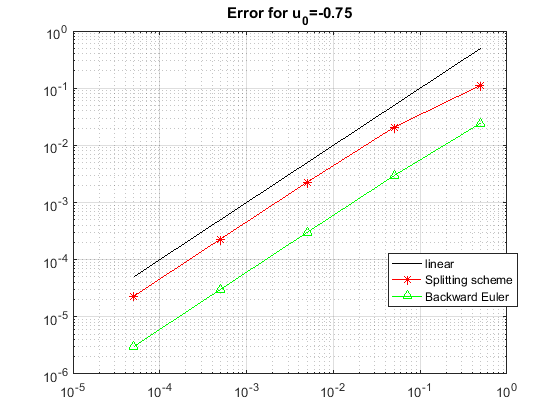
\includegraphics[width=.4\textwidth]{odeplayerrorn075.png}
        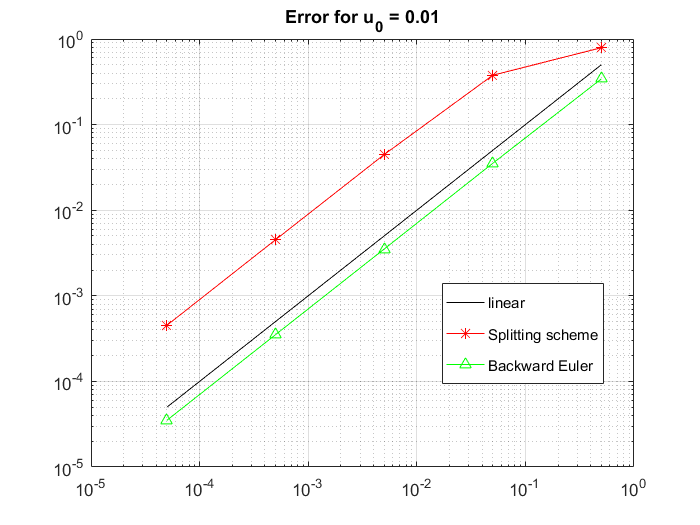
\includegraphics[width=.4\textwidth]{odeplayerror001.png}
		\caption{Error plots for backward Euler and the splitting scheme on loglog graphs. \mpcomment{Define what error means}}
		\label{fig:odeplayerror}
		\end{figure}



 
% Chapter Template

\chapter{Numerical Methods for the Diffusion Equation} % Main chapter title

\label{Chapter3} % Change X to a consecutive number; for referencing this chapter elsewhere, use \ref{ChapterX}
 
%----------------------------------------------------------------------------------------
%	SECTION 1
%----------------------------------------------------------------------------------------

\section{Finite Difference Method for Parabolic PDE's }

%CODE: Heat062017v2.m, fd1d\_heat.m\\
The goal of this document is to look at convergence of finite difference methods for parabolic PDEs of the form 
%%
\begin{subequations} \label{eqn:parabolicPDE}
\begin{eqnarray}
\pd{}{u}{t} - \nabla \cdot(k \nabla u)=f, \;
x \in \Omega, t>0,
\end{eqnarray}
the heat or diffusion equation, where $\Omega$ is open and bounded.  With initial conditions
and boundary conditions:
%%
\begin{eqnarray}
B.C.&\hspace{5mm} u(x,t) =h(t),   &\forall \, x \in \partial\Omega, \, t>0 
\\
I.C.&\hspace{5mm}  u(x,0) = u_0(x) &\forall \, x \in \Omega.
\end{eqnarray}
\end{subequations}
%%
This will be done by looking at two codes. One is a more general code creating during MTH553 at Oregon State University with Professor Adel Faridani Spring 2017. This code allows for implicit, explicit and Crank-Nicolson schemes based on the chosen value of $\mu$. The second code was developed by Professor Peszynska, takes a more in depth look at the implicit method. Some notation differs between methods, but overall methods are very similar.  Both codes use an implicit method that is point centered  difference in space domain and backward difference in time. The error of the implicit and explicit methods is $O(\Delta x^2 + \Delta t)$ and for the Crank-Nicolson  is $O(\Delta x^2 + \Delta t^2)$ .\\
 
%-----------------------------------
%	SUBSECTION 1
%-----------------------------------

\subsection{Multiple Method Code for Equation (\ref{eqn:parabolicPDE}) }
The first code is set up to calculate a numerical solution for 
\begin{subequations}
\begin{eqnarray}
&u_t - k u_{xx} = f(x,t) &x \in (a,b),\, t>0 \\
B.C.&\hspace{5mm} u(a,t) =h_l(t),   \hspace{1cm}   u(b,t) = h_r(t) &t>0
\\
I.C.&\hspace{5mm}  u(x,0) = u_0(x) &x\in(a,b)
\end{eqnarray}
\end{subequations}
where $k$ is a constant. The code is based on the Crank-Nicolson scheme but can be changed to explicit of implicit using the variable $\mu$, where $\mu = 1$ is used for an implicit method, $\mu=0$ for explicit and $\mu = 1/2$ for Crank-Nicolson. The main equation for this scheme is
%
\small
\begin{align} \label{eqn:muparabolicparabolicPDE}
U_j^{n}    - r k\mu\big(U_{j+1}^{n}-2U_j^{n}+U_{j-1}^{n}\big) =&\\
 U_j^{n-1} + rk(1-\mu)&\big(U_{j+1}^{n-1}-2U_j^{n-1}+U_{j-1}^{n-1}\big)
 + \Delta t\big(\mu f_j^{n}+(1-\mu)f_j^{n-1}\big), 
\label{equ matrix Q} \nonumber 
\end{align}
\normalsize
%%
where $r=\frac{\Delta t}{(\Delta x)^2}$. Letting $B$ be the matrix representation of the left hand side of \ref{eqn:muparabolicparabolicPDE} such that $BU^n$ gives the corresponding $j$th component, we get the the following tridiagonal matrix, 
\begin{eqnarray}
B = \begin{bmatrix} 
1+\mu 2 r k & -\mu r k  \\
-\mu r k       & 1+\mu 2 r k& -\mu r k  \\
                    & \ddots           & \ddots & \ddots \\
            & &        -\mu r k  &  1+\mu 2 r k &  -\mu r k  \\
                      &   & &        -\mu r k  &  1+\mu 2 r k   \\
\end{bmatrix},
\end{eqnarray}
we can then write the scheme as 
\begin{eqnarray}
BU^{n} &=& {R}^{n-1}, 
\end{eqnarray}
where both $R$ and $B$ are dependent on $\mu$ and $R$ stands for the right hand side and not to be confused with the residual. Let
\begin{eqnarray}
U^{n} = \begin{bmatrix}
U_1^{n}\\
\vdots\\
U_N^{n}\\
\end{bmatrix}
\hspace{1cm} \text{ and }\hspace{1cm}
{R}^{n-1} = \begin{bmatrix}
R_1^{n-1}\\
\vdots\\
R_N^{n-1}\\
\end{bmatrix}
\end{eqnarray}
where $N$ is the number of time steps subtract 1, i.e. then numbers of points used in the space dimension excluding the boundary points.  
In the code, a matrix $Q$ was used to help calculate $R^{n-1}_j$ in equation  \ref{eqn:matrixQFIparabolicPDE} for $j=1,\dots,N$,
\begin{eqnarray}
Q = \begin{bmatrix} \label{eqn:matrixQFIparabolicPDE}
1-2 r k (1-\mu) & r k (1-\mu)  \\
 r k (1-\mu)        & 1-2 r k (1-\mu) &  r k (1-\mu)   \\
                    & \ddots           & \ddots & \ddots \\
            & &         r k (1-\mu)   &1-2 r k (1-\mu)  &  r k (1-\mu) \\
                      &   & &       r k (1-\mu) &  1-2 r k (1-\mu)    \\
\end{bmatrix}.
\end{eqnarray}

Both $A$ and $Q$ are $N\times N$ matrices.  A vector, $P$, was used to incorporate the boundary conditions 
\begin{eqnarray}
P= 
\begin{bmatrix}
\mu r k g(t_{n}) + r k (1-\mu) h_l(t_{n-1})\\
0\\
\vdots \\
0 \\
\mu r k h(t_{}) n+ r k (1-\mu) h_r(t_{n-1})
\end{bmatrix}.
\end{eqnarray}
The vector $R^{n-1}$ is then calculated using $Q$, $P$, the right hand side equation, $f$, as seen in equation \ref{equn Rm} below. In equation \ref{equn Rm}, $x$ is a vector of the interior  points, length $N$.  Then $R^{n-1}$ and matrix $A$ are used to calculate $U^{n}$ in equation \ref{equn Un}
\begin{eqnarray}
 R^{n-1} &=& QU^{n-1}+P+\Delta t(\mu f(x,t_{n}) +(1-\mu)f(x,t_{n-1}) )\label{equn Rm}\\
    U^{n}& =& B^{-1}R^{n-1} \label{equn Un}.
\end{eqnarray}
The code steps through this process until the specified end time is reached. 
%-----------------------------------
%	SUBSECTION 2
%-----------------------------------
\subsection{Fully Implicit Code for Equation (\ref{eqn:parabolicPDE})}
The main differences between this and the previous method are the way the boundary conditions are implemented and that this method is only implemented fully implicitly. The second code used was provided by Professor Peszynska. The code uses the implicit method to calculate a finite difference approximation of a simple  parabolic two-point boundary value problem $u_t-u_{xx} = f$ as a function with imputes $M, a, b, u_a, u_b, T, dt$ correspondingly number of $x$ steps, left end point, right end point, left boundary condition, right boundary condition, final time and time step size. This code calculates the error and graphs the function as well as showing the first few time step changes. Note that the boundary conditions are treated differently. 


\begin{subequations}
	\begin{eqnarray}
	&u_t-k u_{xx} = f  &x \in (a,b),\, t>0 \label{eqn:DiffusionDir} \\
	B.C.&\hspace{5mm} u(a,t) =h_l(t) = 0,   \hspace{1cm}   u(b,t) = h_r(t)=0 &t>0
	\\
	I.C.&\hspace{5mm}  u(x,0) = u_0(x) &x\in(a,b)
	\end{eqnarray}
\end{subequations}
were $f$ is a function of both $x$ and $t$.

Writing this as a fully implicit numerical method we get
\begin{eqnarray}
U^{n}_j + k \frac{\mytau}{h^2}(2U^{n}_j-U^{n}_{j-1}-U^{n}_{j+1}) =\mytau f+U^{n-1}_j.
\end{eqnarray} 

Writing this out in matrix form we have.

\begin{eqnarray} \label{eqn. impl sch}
 \left( \begin{bmatrix}
	1 &  &  &  &  \\
	& 1 &  &  &  \\
	&  & \ddots &  &  \\
	&  &  & 1 &  \\
	&  &  &  & 1 
	\end{bmatrix}  
	- k \frac{ \mytau}{h^2}  \begin{bmatrix}
	0 &  &  &  &  \\
	1 & -2 & 1 &  &  \\
	& \ddots & \ddots & \ddots &  \\
	&  & 1 & -2 & 1 \\
	&  &  &  &  0
	\end{bmatrix}  \right) \begin{bmatrix}
U^{n}_1 \\
U^{n}_2 \\
\vdots\\
U^{n}_{M}\\
U^{n}_{M+1}

\end{bmatrix}  
= 
 \begin{bmatrix}
0 \\
\mytau f \\
\vdots\\
\mytau f \\
0
\end{bmatrix}  
+
 \begin{bmatrix}
0 \\
U^{n-1}_2 \\
\vdots\\
U^{n-1}_{M} \\
0 
\end{bmatrix} 
\end{eqnarray}

and let 
\begin{center}
$ B = \begin{bmatrix}
1 &  &  & & \\
-k \frac{\mytau}{h^2} & 1+2 k \frac{\mytau}{h^2} & -k \frac{\mytau}{h^2} & & \\
& \ddots & \ddots & \ddots \\
& &-k \frac{\mytau}{h^2} & 1+2 k \frac{\mytau}{h^2} & -k \frac{\mytau}{h^2}   \\
& &  &  & 1 
\end{bmatrix}  $
\end{center}
then if $C$ is a vector of length $M$ with $c$ in all entries except the first and last entries which are zero. Then equation (\ref{eqn. impl sch}) can be rewritten as
\begin{eqnarray}
 B U^{n} = \mytau f(\mathbf{x},t_n) +U^{n-1}.
\end{eqnarray}
Where $\mathbf{x}$ is the containing all $x$ nodes. 

For $g(u)=1$, i.e. $c=-1$, the numerical solution for two values of $\varepsilon$ and the initial value is shown in Figure \ref{fig:FIdirBCex1}. For this example $a=0$, $b=1$, $t_{final}=1$ and $\mytau = h^2$.  Figure \ref{fig:FIdirBCex1} was created in Matlab using the build in $\setminus$ function,
\begin{eqnarray} \label{eqn. ACSolveForUn}
 U^{n} = B \setminus \left( \mytau f(\mathbf{x},t_n)  +U^{n-1} \right)
\end{eqnarray}
for each time step.  %%% code:  Cahn_Allenv4_3 and Cahn_Allenv4_Comparison1

		\begin{figure}[H]
		\centering
		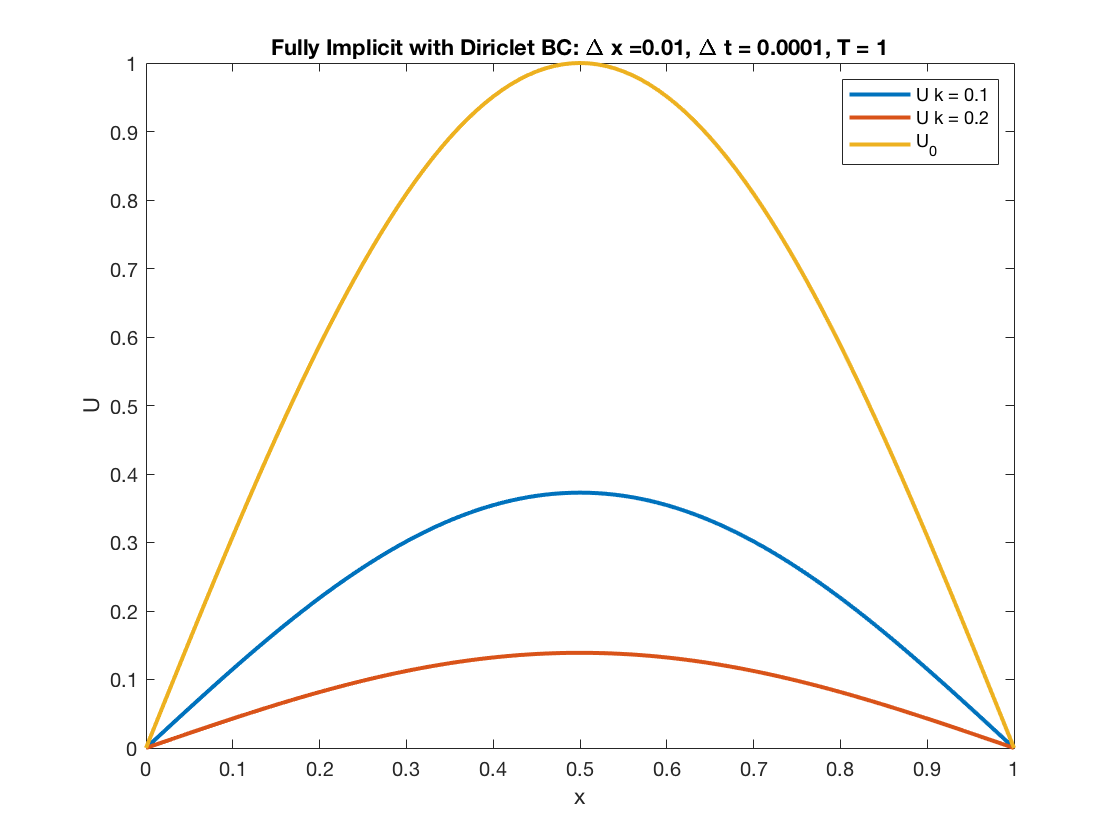
\includegraphics[width=.6\textwidth]{FIdirBCex1.png}
		\caption{Numerical solution using fully implicit finite difference code for the linear diffusion equation where $f=0$, $a=0$, $b=1$, $T=t_{final}=1$, $u_0 = \sin(\pi x) $. Plotted are numerical solutions for two diffusion coefficients, $k=0.1$ and $k=0.2$.}
		\label{fig:FIdirBCex1}
		\end{figure}


%-----------------------------------
%	SUBSECTION 3
%-----------------------------------
\subsection{Convergence Results}
% CODE: Heat062017v2.m, fd1d\_heat.m\\
The first example used was the basic example $u_t-u_{xx}=0$, $u(x,0)=u_{int}(x)= \sin(\pi x) e^{- \pi^2 t}$ on $(0,1)$ and $u|_{\partial u} = u_D=0$. Note that the notation differs between methods.  and the max difference for each graph is listed below the graph.

	Table \ref{tab:conv1} below shows the error and calculated order of accuracy for $h$, $\alpha$ for given $h$ and $\tau$ using the first code with $\mu = 1$ for an implicit method. These values were compared to the second code The error value $e_{\infty}$ was calculated using the known solution, $\hat{U}=U_{exact}$.  In words, $e_{\infty} $ was calculated by taking the maximum absolute difference at each time step then taking the maximum of all the time steps. In symbols, $e_{\infty} = \max_n \max_j  |\hat{U}_j^n-U_j^n|.$ The order of accuracy was calculated using 
	$$\alpha_2 = \frac{\log e_1-\log e_2}{\log h_1 - \log h_2}$$
	where the lower index refers to the row of the value.  \\
	\indent \textbf{Q:} Why are we using $h$ and not $\tau$ to calculate $\alpha$? 
    \\
    For optimal convergence you set $\tau$ to depend on $h$ in some predefined way, so there is only one parameter.\\
	\indent \textbf{Q:} Is there an optimal way to space $h$ efficiently calculate $\alpha$? 
    \\
    The easiest way for ``eyeball'' convergence order checking is to space $h$ with a factor of 10. But any other way will work.
    \\
	In the table $\tau \sim h^2$. The first two values were the same for both methods, the third error value in the table was calculated using just the second code since the first took too long to compile. 
 
 %%%%%%
    \begin{table}[H]
	\begin{center}
		\begin{tabular}{ | c | c | c | c |}
			\hline
			$h$ & $\tau$ & $e_{\infty} $ & $\alpha$ \\ 
			\hline
			 0.1 & 0.01 & 0.0203 & - \\  
			\hline
			 0.01 & 0.0001 &  2.1171e-04 & 1.9822   \\
			 \hline
			 0.001 & 1.00e-06 &  2.1180e-06 &  1.9998  \\
			\hline
		\end{tabular}
        \caption{Error results of max norm.}
        \label{tab:conv1}
	\end{center}
\end{table}
%%

Table \ref{tab:conv2} shows the error results of the $\ell_2$ norm in both time and space numbers. These numbers were calculated using the built in norm function in MATLAB. 
 \begin{table}[H]
	\begin{center}

		\begin{tabular}{ | c | c | c | c |}
			\hline
			$h$ & $\tau$ & $e_{2} $ & $\alpha$ \\ 
			\hline
			0.1 & 0.01 & 0.06308 & - \\  
			\hline
			0.01 & 0.0001 &  0.006477 &  0.9889  \\
			\hline
			0.001 & 1.00e-06 &  0.0205 &   0.4999 \\
			\hline
		\end{tabular}
        \caption{Error results of $\ell_2$ norm}    
        \label{tab:conv2} 
	\end{center}
   \end{table}
   
%----------------------------------------------------------------------------------------
%	SECTION 2
%----------------------------------------------------------------------------------------
   
   \section{Nonlinear Diffusion Equation, Fully Implicit}
   %
%-----------------------------------
%	SUBSECTION 1
%-----------------------------------
\subsection{Nonlinear Diffusion Equation with Dirichlet Boundary Conditions}
   In preparation to work with the phase field model, this section will discuss nonlinear diffusion equations of the form 
%
\begin{subequations}
	\begin{eqnarray}
	&u_t-\varepsilon u_{xx}+\frac{1}{\varepsilon}g(u) = f  &x \in (a,b),\, t>0 \label{eqn. ACexmple} \\
	B.C.&\hspace{5mm} u(a,t) =h_l(t) = 0,   \hspace{1cm}   u(b,t) = h_r(t)=0 &t>0
	\\
	I.C.&\hspace{5mm}  u(x,0) = u_0(x) &x\in(a,b)
	\end{eqnarray}
\end{subequations}
were $f$ is a function of both $x$ and $t$ and $\varepsilon$ is a scalar constant. The first example that will be discussed will have $f = 0$. The discretization used for this problem was a fully implicit method,
\begin{eqnarray}
U^{n}_j-U^{n-1}_j + \varepsilon\frac{ \mytau}{h^2}(2U^{n}_j-U^{n}_{j-1}-U^{n}_{j+1})+\frac{\mytau}{\varepsilon}g(U^n_j) =0 \label{eqn. DirImpHomCA},
\end{eqnarray} 
where $h = \frac{b-a}{M}$ is the uniform step size in space and thus $j=1,\dots,M+1$. Then in the time domain, $\mytau$ is the uniform step size. 


Next, we consider when $g(u)$ is not constant and $f \ne 0$. For example, 
\begin{subequations}
	\begin{eqnarray}
	&u_t-\varepsilon u_{xx}+\frac{1}{\varepsilon}g(u) = f  &x \in (0,1),\, t>0  \\
	B.C.&\hspace{5mm} u(0,t) = 0,   \hspace{2cm}   u(1,t) =0 &t>0
	\\
	I.C.&\hspace{5mm}  u(x,0) = u_0(x)=sin(\pi x) &x\in(0,1)
	\end{eqnarray}
\end{subequations}
%
where 
\begin{subequations}
\begin{align}
 g(u) =& u^3-u \\
 f(x,t) =& \sin(\pi x)+\varepsilon \pi^2 (t+1) \sin(\pi x) \\ & \hspace{3cm}+\frac{1}{\varepsilon} \Big((t+1)\sin(\pi x)-\big((t+1)\sin(\pi x)\big)^3\Big).
\end{align}
\end{subequations}
%
The exact solution for this system of equations is 
\begin{eqnarray}
u = (t+1)\sin(\pi x).
\end{eqnarray} 
Because $g(u)$ is not linear in $u$, using a fully implicit scheme requires an iterative method. Consider the method in (\ref{eqn. CahnAllenNewton})
\begin{eqnarray} \label{eqn. CahnAllenNewton}
U^{n}_j-U^{n-1}_j + \varepsilon \frac{ \mytau}{h^2}(2U^{n_k}_j-U^{n_k}_{j-1}-U^{n_k}_{j+1})+\frac{\mytau}{\varepsilon}g(U^{n_k}_j) = \mytau f,
\end{eqnarray} 
where $f = f(x_j,t_n)$ and $n_k$ represents the time step and the Newton iteration, i.e. $n$ is the time step and the subscript $k$ is the Newton iteration. For detail on Newton's Method see section \ref{Sect:Newton'sMethod}. The initial guess used at each time step was the previous time step, $n-1$, so $U^{n_0} = U^{n-1}$. The 2-grid-norm was used to calculate the norm of the residual. In this case the accuracy was set to $10e{-12}$, thus the norm of the residual needed to be less $10e{-12}$ in order for the current iteration to be accepted as the numerical solution. The tolerance and the max iterations were set leniently at 100 and 25 respectively.  

The residual, in this case, for the interior spacial notes is
\begin{eqnarray}
R_j^{n_k} = U^{n}_j-U^{n-1}_j + \varepsilon \frac{ \mytau}{h^2}(2U^{n_k}_j-U^{n_k}_{j-1}-U^{n_k}_{j+1})+\frac{\mytau}{\varepsilon}g(U^{n_k}_j) - \mytau f(x_j,t_n)
\end{eqnarray}
and for the boundary

\begin{align}
R_{1}^{n_k} =& U_1^{n_{k}}-u(x_1,t_n) \\
R_{M+1}^{n_k} =& U_{M+1}^{n_k} - u(x_{M+1},t_n) 
\end{align}
In this case $u(x_1,t_n) =  u(x_{M+1},t_n) =0$ for all $t_n >0$. The Jacobian is as follows
\begin{center}
$ J = \begin{bmatrix}
1 &  &  & & \\
-\varepsilon \frac{\mytau}{h^2} & 1+2 \varepsilon \frac{\mytau}{h^2} +\frac{1}{\varepsilon}g'(U_2^{n_k})& -\varepsilon \frac{\mytau}{h^2} & & \\
& \ddots & \ddots & \ddots \\
& &-\varepsilon \frac{\mytau}{h^2} & 1+2 \varepsilon \frac{\mytau}{h^2} +\frac{1}{\varepsilon}g'(U_M^{n_k})& -\varepsilon \frac{\mytau}{h^2}   \\
& &  &  & 1 
\end{bmatrix}.  $
\end{center}


%
%-----------------------------------
%	SUBSECTION 2
%-----------------------------------
\subsection{Nonlinear Diffusion Equation with Neumann Boundary Conditions}

%Code: Cahn_Allenv7_2
The boundary condition is the only thing that differs between Allen-Cahn heat equation fully implicit with Neumann boundary condition method and the fully implicit method with Dirichlet boundary conditions. The initial boundary value problem now becomes
\begin{subequations}
	\begin{eqnarray}
	&u_t-\varepsilon u_{xx}+\frac{1}{\varepsilon}g(u) = f  &x \in (a,b),\, t>0  \\
	B.C.&\hspace{5mm} u'(a,t) = 0,   \hspace{5mm}   u'(b,t) =0 &t>0
	\\
	I.C.&\hspace{5mm}  u(x,0) = u_0(x) &x\in(a,b)
	\end{eqnarray}
\end{subequations}

There are only a couple of changes between the code for Neumann and Dirichlet boundary condition. The change are, the boundary conditions and the Jacobian. In the code, this is what differs for the boundary conditions. First is the center followed by the boundary conditions
\begin{eqnarray}
R_j^{n_k} = U^{n}_j-U^{n-1}_j + \varepsilon \frac{ \mytau}{h^2}(2U^{n_k}_j-U^{n_k}_{j-1}-U^{n_k}_{j+1})+\frac{\mytau}{\varepsilon}g(U^{n_k}_j) - \mytau f(x_j,t_n)
\end{eqnarray}
and for the boundary
\begin{align}
R_{1}^{n_k} =& U_1^{n_{k}}+\varepsilon \frac{\mytau}{h^2} (2 U_1^{n_k}-2 U_2^{n_k}) +\frac{\mytau}{\varepsilon} g(U_1^{n_k})-\mytau f(x_1,t_n)-U_1^{n-1}\\ 
R_{M+1}^{n_k} =& U_{M+1}^{n_k}+\varepsilon \frac{\mytau}{h^2} (2 U_{M+1}^{n_k}-2 U_{M}^{n_k})+\frac{\mytau}{\varepsilon} g(U_{M+1}^{n_k})-\mytau f(x_{M+1},t_n)-U_{M+1}^{n-1}
\end{align}
The Jacobain for this method is
\scriptsize{
\begin{center}
$ J = \begin{bmatrix}
1+2\varepsilon \frac{\mytau}{h^2}+\frac{\mytau}{\varepsilon} g'(U_1^{n_k})  & -2\varepsilon \frac{\mytau}{h^2} &  & & \\
-\varepsilon \frac{\mytau}{h^2} & 1+2 \varepsilon \frac{\mytau}{h^2} +\frac{1}{\varepsilon}g'(U_2^{n_k})& -\varepsilon \frac{\mytau}{h^2} & & \\
& \ddots & \ddots & \ddots \\
& &-\varepsilon \frac{\mytau}{h^2} & 1+2 \varepsilon \frac{\mytau}{h^2} +\frac{1}{\varepsilon}g'(U_M^{n_k})& -\varepsilon \frac{\mytau}{h^2}   \\
& &  &  -2\varepsilon \frac{\mytau}{h^2} & 1+2\varepsilon \frac{\mytau}{h^2}+\frac{\mytau}{\varepsilon} g'(U_{M+1}^{n_k}) 
\end{bmatrix}.  $
\end{center} }
\normalsize


%----------------------------------------------------------------------------------------
%	SECTION 3
%----------------------------------------------------------------------------------------
\section{Nonlinear Diffusion Equation, Time Lagging}
%
For the time lagging method, the function $g(u)$ is evaluated at $U^{n-1}$, thus equation (\ref{eqn. CahnAllenNewton}) becomes
\begin{eqnarray} \label{eqn. CahnAllenTimeLagging}
U^{n}_j-U^{n-1}_j + \varepsilon \frac{ \mytau}{h^2}(2U^n_j-U^n_{j-1}-U^n_{j+1})+\frac{\mytau}{\varepsilon}g(U_j^{n-1} ) =\mytau f.
\end{eqnarray} 
This method does not require an iterative method and can be solved similarly to how it is in equation (\ref{eqn. ACSolveForUn}), however this method can deviate from the true solution more than the fully implicit method. 


%----------------------------------------------------------------------------------------
%	SECTION 5
%----------------------------------------------------------------------------------------
\section{Allen-Cahn Heat Equation Splitting Method with Neumann Boundary Conditions} \label{Sect. Allen-Cahn Heat Equation Splitting Method with Neumann Boundary Conditions} 
The main idea for the splitting method is to break up the nonlinearity, in our case the $g(u) =u^3-u$, into an expansive and an contractive term and 
evaluate the contractive term implicitly and the expansive term explicitly. This is more explicitly discussed in the section \ref{Sect:Splitting}. The first splitting method used is 
\begin{eqnarray} \label{eqn. CahnAllenSplitting1}
U^{n}_j-U^{n-1}_j + \varepsilon \frac{ \mytau}{h^2}(2U^n_j-U^n_{j-1}-U^n_{j+1})+\frac{\mytau}{\varepsilon}5 U_j^{n}  =\frac{\mytau}{\varepsilon}6 U_j^{n-1}- \frac{\mytau}{\varepsilon}(U_j^{n-1})^3+\mytau f.
\end{eqnarray} 



%----------------------------------------------------------------------------------------
%	SECTION 5
%----------------------------------------------------------------------------------------
\section{Comparing Fully Implicit, Time Lagging, and the Splitting Methods for the Cahn-Allen Heat Equation} \label{Sect. Comparing Fully Implicit, Time Lagging, and the Splitting Methods for the Cahn-Allen Heat Equation} 
This section compared the fully implicit, time lagging, and the splitting methods for the Cahn-Allen heat equation. All methods used Neumann boundary conditions, thus the initial boundary value problem for this section is 
\begin{subequations}
	\begin{eqnarray}
	&u_t-\varepsilon u_{xx}+\frac{1}{\varepsilon}g(u) = f  &x \in (a,b),\, t>0  \\
	B.C.&\hspace{5mm} u'(a,t) = 0,   \hspace{5mm}   u'(b,t) =0 &t>0
	\\
	I.C.&\hspace{5mm}  u(x,0) = u_0(x) &x\in(a,b)
	\end{eqnarray}
\end{subequations}
where unless otherwise specified $a=0$ and $b=1$. This section will looks at a few specific examples with different initial conditions. The first exam will have the initial condition of $u_0\left( (a, \frac{b-a}{2}) \right)= -1$ for the first half of the interval $(0,1)$ and the second half will be one, $u_0\left( [\frac{b-a}{2},b) \right)= 1$. If there are an odd number of nodes, then the middle node is included in the second half and given the initial value one. 
		\begin{figure}[H]
		\centering
		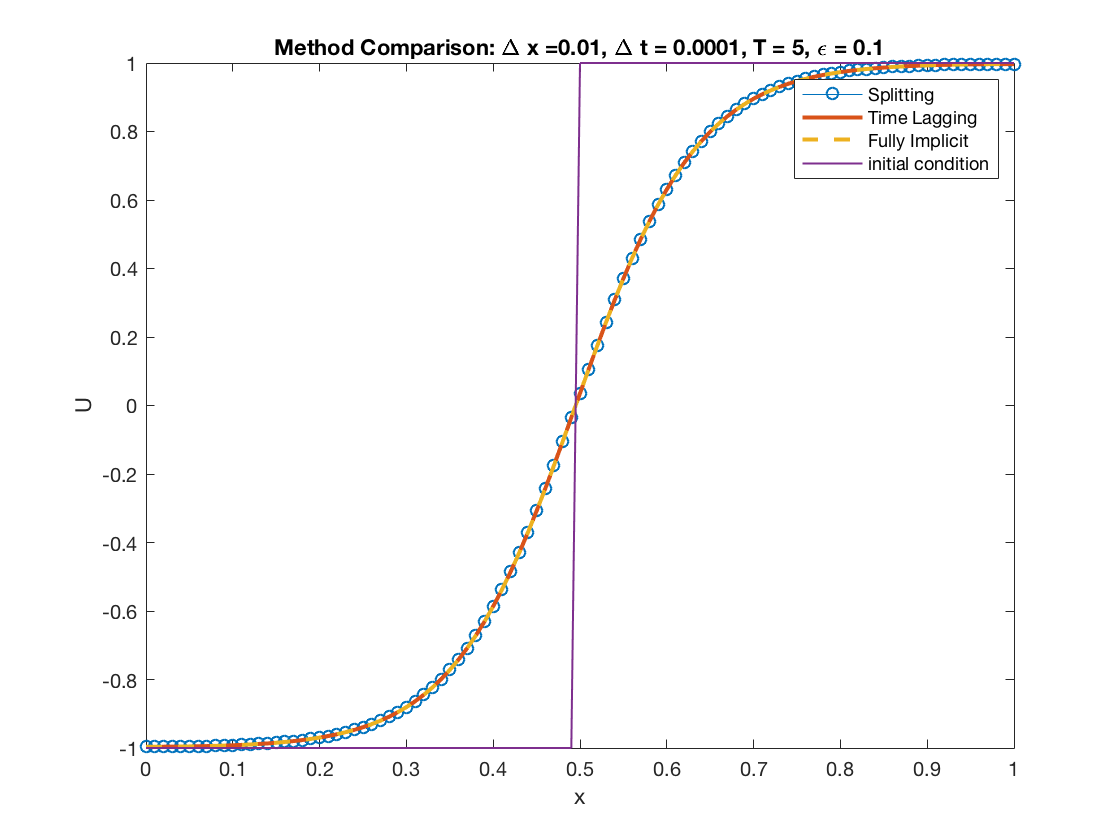
\includegraphics[width=.45\textwidth]{MethComUo1e01.png}
        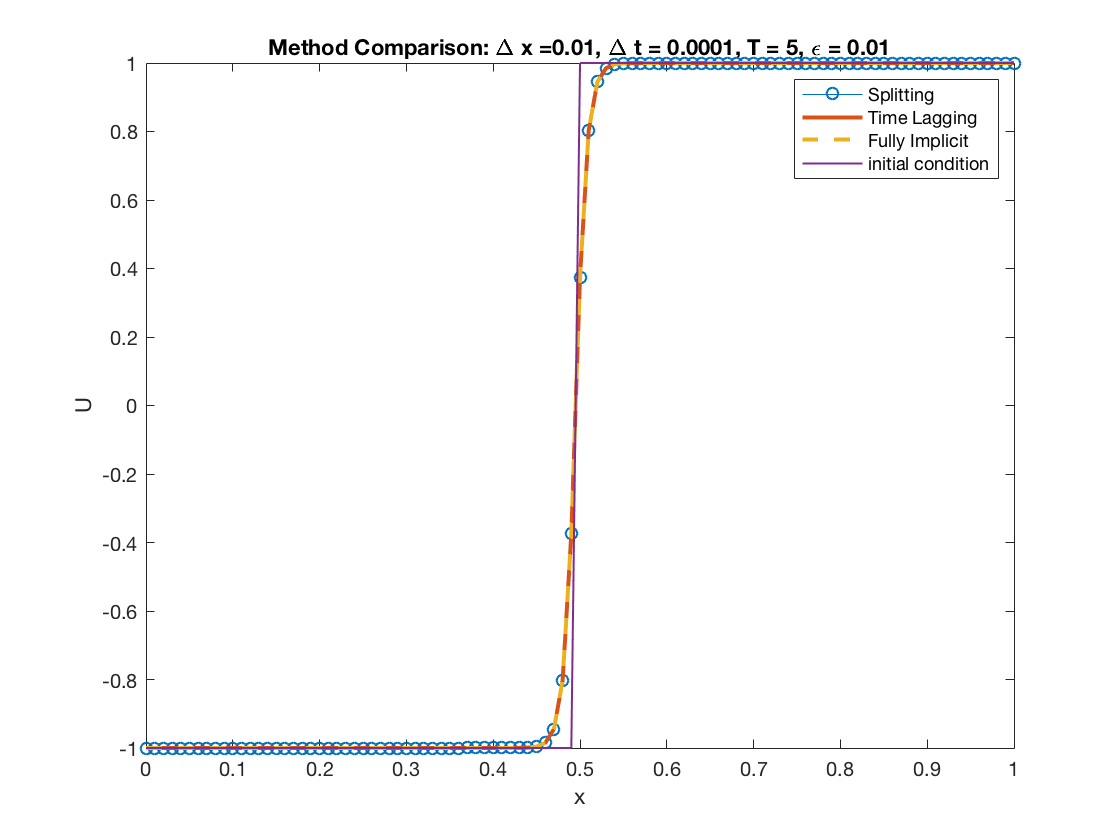
\includegraphics[width=.45\textwidth]{MethComUo1e001.png}
		\caption{Plots for all three methods and two different values of $\varepsilon$ but keeping all other inputs the same. }
		\label{fig:MethComUo1}
		\end{figure}

The initial value for this example was $u_0=\frac{1}{3}\cos(7\pi x )+\frac{1}{3}\cos(29\pi x )+\frac{1}{3} \cos(\pi x)$   
		\begin{figure}[H]
		\centering
		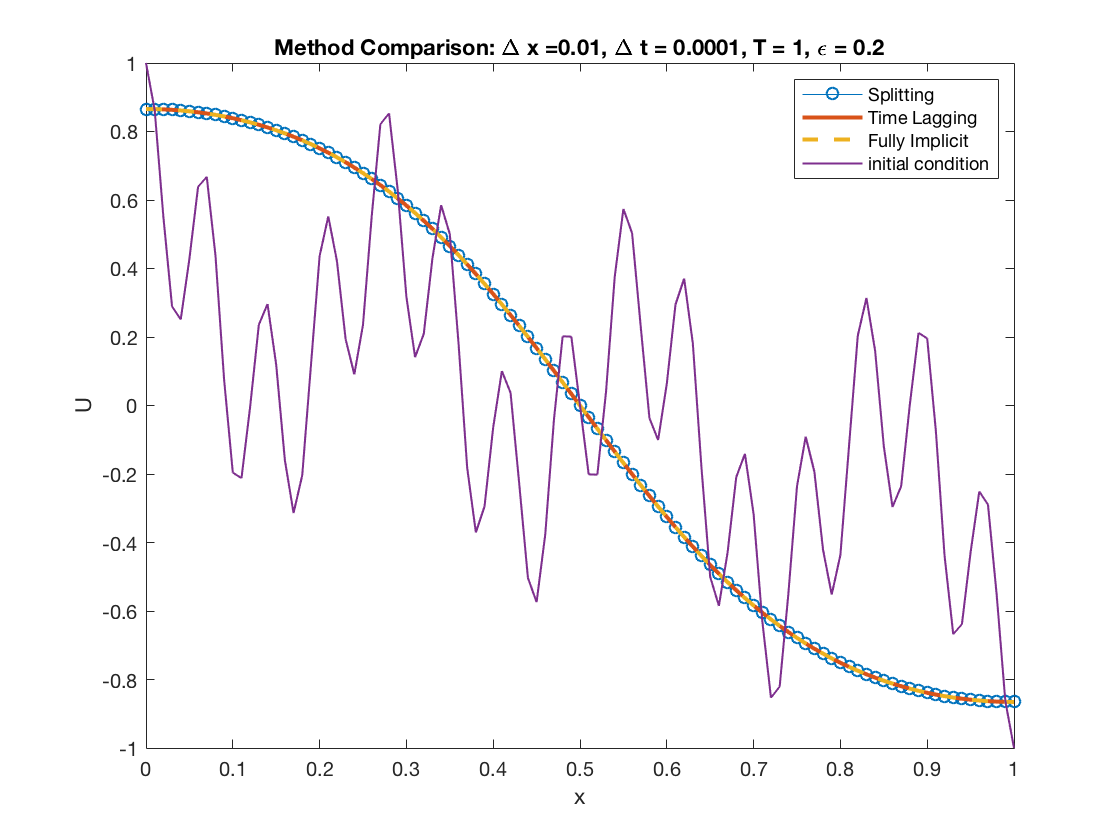
\includegraphics[width=.6\textwidth]{MethComUo2e02.png}
        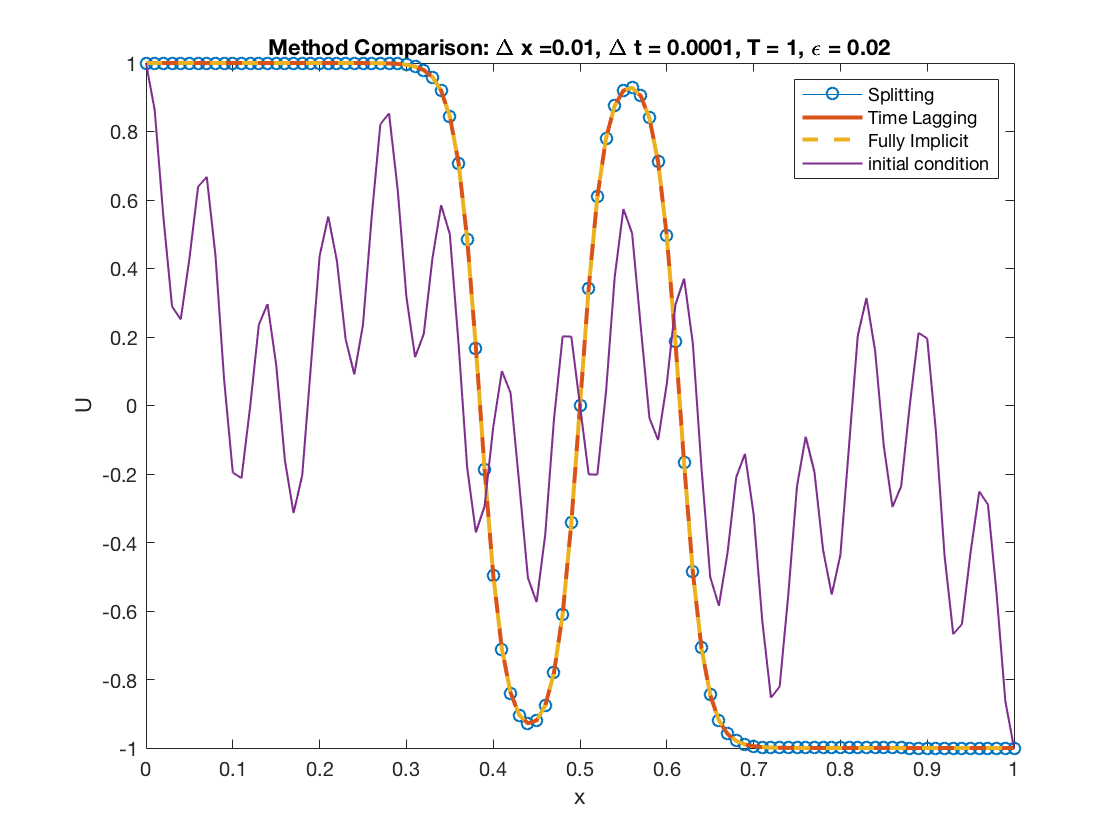
\includegraphics[width=.6\textwidth]{MethComUo2e002.png}
		\caption{Plots for all three methods and two different values of $\varepsilon$ but keeping all other inputs the same. }
		\label{fig:MethComUo2}
		\end{figure}
For the case that $\varepsilon = 0.2$, the $||U_{FI}-U_{S}||_{2, \Delta} = 9.2e{-5}$ while $||U_{FI}-U_{TL}||_{2, \Delta} = 8.0e{-7}$ where $||\cdot||_{2, \Delta}$ is the grid 2-norm and in this case is taken at the final time, $t=T=1$, and $U_{FI}$ is $U_{final}$ using the fully implicit method. 






        
% Chapter 4

\chapter{Phase Field Models} % Main chapter title

\label{Chapter4} % Change X to a consecutive number; for referencing this chapter elsewhere, use \ref{ChapterX}

%----------------------------------------------------------------------------------------
%	SECTION 1
%----------------------------------------------------------------------------------------

\section{Stephan Problem}

The goal of this section is to give an overview the Stephan problem using notation mostly from Guenther and Lee's book, \parencite{GuetherandLee}. The Stephan problem describes change-of-phase problems. The problem addressed in this section will be a phase change between water and ice. At the initial time the problem discussed here consists of an insulated pipe of length two with the left half filled with water and the right half filled with ice with heat applied to just the left end. Let the specific heat, density, thermoconductivity, and temperature of water be denoted respectively by $c_w, \, \rho_w, \,  k_w,$ and $u_w$. Similarly for ice with $i$ instead of $w$. Let $s(t)$ be the location of the ice-water interface at any given time. Our objective is to find the temperature distribution over time, $t>0$. \\
Both the ice section and the water section satisfy the heat equation. Combining the constants, let $a_w=k_w/c_w \rho_w$ and similarly for ice. Then
\begin{eqnarray} \begin{cases} 
\pd{}{u_w}{t}=a_w \pd{2}{u_w}{x}  & 0< x < s(t), \quad t>0 \\
\pd{}{u_i}{t}=a_i \pd{2}{u_i}{x}  & s(t) <x <2, \quad t>0. \label{mainstefanpde}
\end{cases}
\end{eqnarray}

For simplicity the $w$ and $i$ subscripts of $u$ will be dropped. Let the temperature at the ice-water interface be zero, 
\begin{eqnarray}
	u\big|_{s(t)^-}= u\big|_{s(t)^+} =0
\end{eqnarray}
and let
\begin{eqnarray}
	a u_x\big|_{s(t)^-}= a u_x\big|_{s(t)^+}- \mathcal{L}\dot{s}\quad t\ge0
\end{eqnarray}
where $\dot{s}$ is the time derivative of the position of the phase transition. 
Approaching this system in a weak sense, let $\varphi \in C_0^\infty(Q)$ where $Q = (0,2) \times (0,T)$ and $u \in H^1(Q)$. 
Changing notations slightly let 
\begin{subequations}
\begin{eqnarray}
u_t - \grad (k \grad u) = 0 \quad \text{ on } \Omega_1 \cup \Omega_2 \label{equn gradu}\\ 
-[k \grad u \cdot \nu] = \mathcal{L} v \cdot \nu \quad \text{ on } S \label{equn jump}\\ 
u = 0 \quad \text{ on } S
\end{eqnarray}
\end{subequations}
Where $S$ is dependent on $t$ and is the location of the interface denoted as $s(t)$ above. Where $Q = \Omega \times (0,T)$. The spacial bounded domain is denoted as $\Omega$, where $\Omega_i$, $i=1,2$, are the domains of each phase, letting $\Omega_1$ be water and $\Omega_2$ be ice. The location of the phase change $S$ is equal to $S := \partial Q_1 \cap \partial Q_2$. The latent heat is denoted as $\mathcal{L}$ and $v$ is the velocity of the interface, given as $\mathcal{L}$ and $\dot{s}$ respectively. The value $k$ is also set in each $\Omega_i$ and is denoted $a$ above. The vector $\nu$ is the unit vector field normal to $S \cap \Omega \times \{t\}$. Let $n_x$ be the unit normal vector in the spatial domain and $n_t$ be the unit normal vector time. \\
Let $\varphi \in C_0^{\infty} (Q)$ and first consider 
\begin{eqnarray*}
\iint_{Q_1} u_t \varphi dx dt &=& -\iint_{Q_1} u \varphi_t dx dt + \int_{\partial Q_1} u \varphi dS\\
&=& -\iint_{Q_1} u \varphi_t dx dt + \int_{\partial Q_1 \setminus S} u \varphi dS + \int_{S} u \varphi dS \\
&=& -\iint_{Q_1} u \varphi_t dx dt 
\end{eqnarray*}
since $u=0$ on $S$ and $\varphi =0$ on $\partial Q_1 \setminus S$. This holds for $Q_2$ as well. Now to formulate the weak form of the Stefan problem consider summing both domains in equation \ref{equn gradu} and multiplying them by $\varphi$. Denoting $Q_{1,2} := Q_1 \cup Q_2$ we begin with


\begin{align*}
0 =& \iint_{Q_1}  u_t\varphi dx dt  + \iint_{Q_1} - \grad(k \grad u) \varphi dx dt +\iint_{Q_2}  u_t\varphi dx dt  + \iint_{Q_2} - \grad(k \grad u) \varphi dx dt  \\*
=& \iint_{Q_{1,2}}  u_t\varphi dx dt  + \iint_{Q_1} (k \grad u) \grad\varphi dx dt - \int_{\partial Q_1} \varphi(k \grad u) \cdot n_x^1 dS +  \iint_{Q_2} (k \grad u) \grad\varphi dx dt \\*
&  \hspace{10cm}- \int_{\partial Q_2} \varphi (k \grad u)\cdot n^2_x  dS \\*
\end{align*}
calculated using Greens theorem in the spatial domain and $n_x^i$, $i=1,2$, are the normal vectors out of the respective $\Omega_i$ and let $n_x = n_x^1=-n_x^2$. Note as above $\varphi=0$ on the boundaries that are not $S$. Also note that equation \ref{equn jump} can be rewritten noting with $n_x$ instead of $\nu$, thus

\begin{eqnarray*}
0 &=& \iint_{Q_{1,2}}  u_t\varphi dx dt  + \iint_{Q_1} (k \grad u) \grad\varphi dx dt - \int_{\partial Q_1} \varphi(k \grad u) \cdot n_x dS + \iint_{Q_2} (k \grad u) \grad\varphi dx dt \\*
& & \hspace{10cm}+ \int_{\partial Q_2} \varphi (k \grad u)\cdot n_x  dS \\*
&=& \iint_{Q_{1,2}}  u_t\varphi dx dt  + \iint_{Q_1} (k \grad u) \grad\varphi dx dt + \iint_{Q_2} (k \grad u) \grad\varphi dx dt+ \int_{S} -\varphi[(k \grad u) \cdot n_x] dS  \\*
&=& \iint_{Q_{1,2}}  u_t\varphi dx dt  + \iint_{Q_{1,2}} (k \grad u) \grad\varphi dx dt +  \int_{S} \varphi \mathcal{L} v \cdot n_x dS.  
\end{eqnarray*}
Now consider how $v \cdot n_x$ can be rewritten, buy starting with derivative of $u$ on $S$ which is constant. Thus,
\begin{eqnarray}
0 &=& \frac{d}{dt} u(x(t),t)\\
&=& \grad_x u \cdot \frac{dx}{dt} + u_t  
\end{eqnarray}
where $\frac{dx}{dt} = v$. Normalizing this vector by $||(\grad_x u, u_t)||_{L_2}$ gives a unit vector normal to the spacial and time domains thus
\begin{eqnarray}
0 = v \cdot n_x + n_t. 
\end{eqnarray}
Using this relation and the fact the the jump of the heavyside function, $[H(u)]$ is one at $S$ we get

\begin{eqnarray*}
0 &=& \iint_{Q_{1,2}}  u_t\varphi dx dt  + \iint_{Q_{1,2}} (k \grad u) \grad\varphi dx dt +  \int_{S} \varphi \mathcal{L} v \cdot n_x dS \\*
&=& \iint_{Q_{1,2}}  u_t\varphi dx dt  + \iint_{Q_{1,2}} (k \grad u) \grad\varphi dx dt -  \int_{S} \varphi \mathcal{L} n_t dS  \\*
&=& \iint_{Q_{1,2}}  u_t\varphi dx dt  + \iint_{Q_{1,2}} (k \grad u) \grad\varphi dx dt -  \int_{S} \varphi \mathcal{L} [H(u)] n_t dS.  
\end{eqnarray*}
Rewriting the normal in time into $n_t=n_t^1 = -n_t^2$ we get
\begin{eqnarray*}
0 &=& \iint_{Q_{1,2}}  u_t\varphi dx dt  + \iint_{Q_{1,2}} (k \grad u) \grad\varphi dx dt -  \int_{S} \varphi \mathcal{L} [H(u)] n_t^1 dS\\*
&=& \iint_{Q_{1,2}}  u_t\varphi dx dt  + \iint_{Q_{1,2}} (k \grad u) \grad\varphi dx dt  -  \int_{\partial Q_1} \varphi \mathcal{L} H(u) n_t^1 dS +\int_{\partial Q_2} \varphi \mathcal{L} H(u) n_t^1 dS\\*
&=& \iint_{Q_{1,2}}  u_t\varphi dx dt  + \iint_{Q_{1,2}} (k \grad u) \grad\varphi dx dt  -  \int_{\partial Q_1} \varphi \mathcal{L} H(u) n_t^1 dS -\int_{\partial Q_2} \varphi \mathcal{L} H(u) n_t^2 dS.\\*
\end{eqnarray*}

Since $H(u)$ is constant on $Q_1$ and $Q_2$, we have $(H(u))_t = 0$ on $Q_1$ and $Q_2$. Adding two integrals that equate to zero gives 
\begin{eqnarray*}
0  &=& \iint_{Q_{1,2}}  u_t\varphi dx dt  + \iint_{Q_{1,2}} (k \grad u) \grad\varphi dx dt  -  \int_{\partial Q_1} \varphi \mathcal{L} H(u) n_t^1 dS -\int_{\partial Q_2} \varphi \mathcal{L} H(u) n_t^2 dS\\*
 &=& \iint_{Q_{1,2}}  u_t\varphi dx dt  + \iint_{Q_{1,2}} (k \grad u) \grad\varphi dx dt  +\iint_{Q_1} \mathcal{L} (H(u))_t \varphi dx dt  -  \int_{\partial Q_1} \varphi \mathcal{L} H(u) n_t^1 dS \\* 
 & &   \hspace{6cm}  +\iint_{Q_2} \mathcal{L} (H(u))_t \varphi dx dt -\int_{\partial Q_2} \varphi \mathcal{L} H(u) n_t^2 dS\\*
 &=&- \iint_{Q_{1,2}}  u\varphi_t dx dt  + \iint_{Q_{1,2}} (k \grad u) \grad\varphi dx dt  -\iint_{Q_1\cup Q_2} \mathcal{L} (H(u)) \varphi_t dx dt \\*
 &=&- \iint_{Q_{1,2}} (u+ \mathcal{L} H(u)) \varphi_t dx dt  + \iint_{Q_{1,2}} (k \grad u) \grad\varphi dx dt  \\*
  &=& \iint_{Q_{1,2}} (u+ \mathcal{L} H(u))_t \varphi dx dt  - \iint_{Q_{1,2}} \grad(k \grad u) \varphi dx dt.  
\end{eqnarray*}
Implying that in the weak sense



\begin{eqnarray}
\big(u+ \mathcal{L} H(u)\big)_t - \grad (k \grad u) = 0.
\end{eqnarray}\\
\vspace{2mm} 

%----------------------------------------------------------------------------------------
%	SECTION 2
%----------------------------------------------------------------------------------------

\section{Phase Field Model}

Derived from the Allen-Cahn equations and physical properties the governing equation for the phase field model is 

\begin{eqnarray}
\phi_t + \frac{1}{\varepsilon}g(\phi) - \varepsilon \Delta \phi =f
\end{eqnarray}
with suitable boundary and initial conditions, where $g(\phi) = \pd{}{G}{\phi}$ and $G$ is the double well potential. Consider a smooth double well potential, $G= (\phi^2-1)^2/4$ then $g = \phi^3 -\phi$. This double well potential has stable equilibria at $x=-1$ and $x=1$ and an unequal equilibrium at $x=0$.

%----------------------------------------------------------------------------------------
%	SECTION 3
%----------------------------------------------------------------------------------------

\section{Phase Field and Temperature Coupled System}

\begin{eqnarray}
\begin{cases}
\phi_t + \frac{1}{\varepsilon}g(\phi) - \varepsilon \Delta \phi =\Lc T\\
\pd{}{}{t}\left(T+\frac{\Lc}{2} \phi \right) - \grad \cdot (D \grad T) = 0
\end{cases}
\end{eqnarray}

                                      
%\include{Chapters/Chapter5} 

%----------------------------------------------------------------------------------------
%	THESIS CONTENT - APPENDICES
%----------------------------------------------------------------------------------------

\appendix % Cue to tell LaTeX that the following "chapters" are Appendices

% Include the appendices of the thesis as separate files from the Appendices folder
% Uncomment the lines as you write the Appendices

% Appendix A

\chapter{Frequently Asked Questions} % Main appendix title

\label{AppendixA} % For referencing this appendix elsewhere, use \ref{AppendixA}

\section{How do I change the colors of links?}

The color of links can be changed to your liking using:

{\small\verb!\hypersetup{urlcolor=red}!}, or

{\small\verb!\hypersetup{citecolor=green}!}, or

{\small\verb!\hypersetup{allcolor=blue}!}.

\noindent If you want to completely hide the links, you can use:

{\small\verb!\hypersetup{allcolors=.}!}, or even better: 

{\small\verb!\hypersetup{hidelinks}!}.

\noindent If you want to have obvious links in the PDF but not the printed text, use:

{\small\verb!\hypersetup{colorlinks=false}!}.

%\include{Appendices/AppendixB}
%\include{Appendices/AppendixC}

%----------------------------------------------------------------------------------------
%	BIBLIOGRAPHY
%----------------------------------------------------------------------------------------

\printbibliography[heading=bibintoc]

%----------------------------------------------------------------------------------------

\end{document}  
